\documentclass[]{exam}
\usepackage{epic,array,ecltree,url,calrsfs}
\usepackage[nointegrals]{wasysym}

%These tell TeX which packages to use.
\usepackage{array,epsfig}
\usepackage{amsmath}
\usepackage{amsfonts}
\usepackage{amssymb}
\usepackage{amsxtra}
\usepackage{amsthm}
\usepackage{mlextra} % must come after ams packages
\usepackage{mathrsfs}
\usepackage[dvipsnames]{xcolor}
\usepackage{array}
\usepackage{graphicx}
\graphicspath{ {../art/} }
\usepackage{bm}
\usepackage{tikz}
\usepackage{multicol}
\usepackage{enumitem}
\setitemize{noitemsep,topsep=0pt,parsep=0pt,partopsep=0pt}

\newcommand{\twonode}{%
  \begingroup\normalfont
  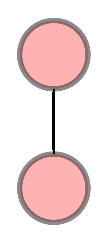
\includegraphics[height=\fontcharht\font`\b]{2nodetree.eps}%
  \endgroup
}

\newcommand{\tf}[1][{}]{%
\fillin[#1][0.25in]%
}

\title{Lab 6: Complexity, Resolution, DPLL}
\author{Foundations of Computer Science}
\date{\today}
%\pagestyle{empty} 
%\footer{}{\thepage}{}
\unframedsolutions
\SolutionEmphasis{\itshape\small}
\SolutionEmphasis{\color{NavyBlue}}


\begin{document}

\maketitle

\setlength{\columnseprule}{1pt}
\begin{questions} 
\section*{Complexity}
\question If a problem $A$ is in $\id{NP}$, its complement is in \fillin[$\id{CoNP}$].
\question Informally, we say $A$ is $\id{NP}$-Hard iff it is \fillin all problems in $\id{NP}$.
\begin{checkboxes}
\choice harder than
\choice as hard as
\CorrectChoice at least as hard as
\choice no harder than
\end{checkboxes}

\question \tf[F] (T/F) If $A$ is $\id{NP}$-Hard, $A$ is in $\id{NP}$.
\question \tf[T] (T/F) If $A$ is $\id{NP}$-Complete, $A$ is in $\id{NP}$.
\question \tf[T] (T/F) If $A$ is $\id{NP}$-Complete, $A$ is $\id{NP}$-Hard.

\question Let $A$ and $B$ be problems such that $A$ is $\id{NP}$-Complete
and $A$ efficiently reduces to $B$. What can we say about $B$?
\begin{checkboxes}
\choice It is smaller than $A$.
\choice It is harder than $A$.
\CorrectChoice It is at least as hard as $A$.
\CorrectChoice It is $\id{NP}$-Hard.
\end{checkboxes}

\clearpage
\section*{Resolution}

\question Consider the following circuit:
\begin{center}
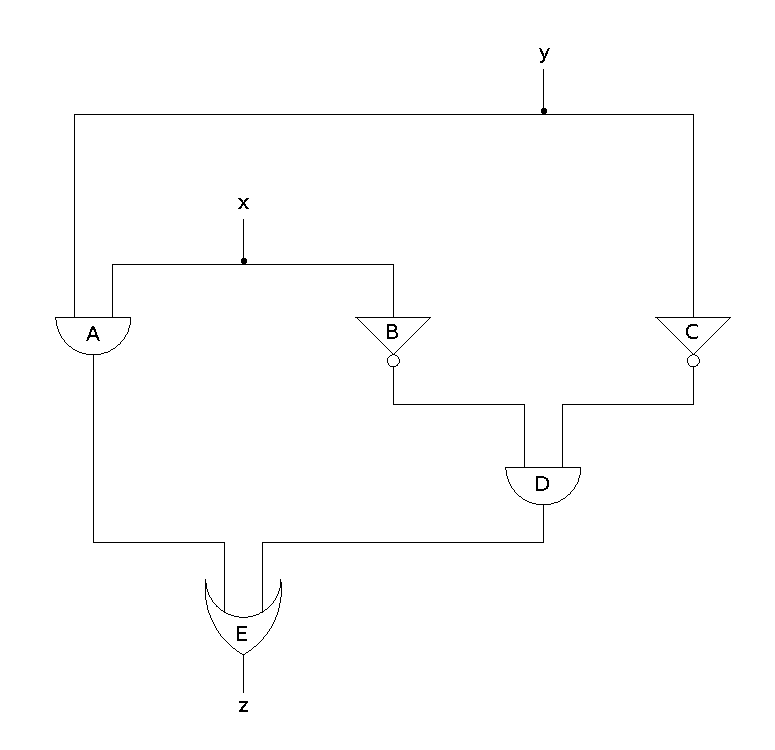
\includegraphics[height=8cm]{equiv_circuit.eps}%
\end{center}

\begin{parts}
\part Write a statement in propositional logic that expresses
$z$ in terms of $x$ and $y$.
\begin{solution}
$z \eqv (x\land y) \lor \ngg (x \land y)$
\end{solution}

\part What logical operator does this circuit implement?
\begin{solution}
$\eqv$
\end{solution}
\end{parts}

\question Transform the set of formulas below into clausal form and refute 
          using resolution.
\[
  \{p,\: p\imp ((q\lor r) \land \ngg (q \land r)),\: p \imp ((s \lor t) \land
      \ngg (s \land t)),\:  s \imp q,\: \ngg r \imp t,\: t \imp s \}
  \]
\begin{solution}
Proceed by changing all formulas to their corresponding CNF. The first formula
is trivial. The second can be converted as follows:
\begin{align*}
&p \imp ((q\lor r) \land \ngg (q \land r))                            && \text{original} & \\
&\equiv \ngg p\lor ((q\lor r) \land \ngg (q \land r))                 && A\imp B \equiv \ngg A \lor B &\\ 
&\equiv \ngg p\lor ((q\lor r) \land (\ngg q \lor \ngg r))             && \text{De Morgan's Laws} &\\  
&\equiv (\ngg p\lor (q\lor r)) \land (\ngg p\lor (\ngg q \lor \ngg r))&& A \lor (B \land C) \equiv (A \lor B) \land (B \lor C)&\\ 
&\equiv (\ngg p\lor q\lor r) \land (\ngg p \lor \ngg q \lor \ngg r)   && \text{associative property} &\\   
&\equiv \{\bar{p}qr, \bar{p}\bar{q}\bar{r} \}                         && \text{clausal form}&\\ 
\end{align*}
The third formula has the same form with different variables, so by the same transformations:
\begin{align*}
&p \imp ((s \lor t) \land \ngg (s \land t)) \\ 
&\equiv \{\bar{p}st, \bar{p}\bar{s}\bar{t} \} \\ 
\end{align*}
The rest of the formulas follow immediately from simple transformations.
Putting these all together in a single set, we have

\[
  \{p, \bar{p}qr, \bar{p}\bar{q}\bar{r}, \bar{p}st, \bar{p}\bar{s}\bar{t}, \bar{s}q, rt, \bar{t}s\}
\]
~\\{ \bf One possible refutation:}
\begin{enumerate}
\item $p,\bar{p}st$: $st$
\item $st,\bar{t}s$: $s$
\item $p,\bar{p}\bar{s}\bar{t}$: $\bar{s}\bar{t}$
\item $s,\bar{s}\bar{t}$: $\bar{t}$
\item $s,\bar{s}q$: $q$
\item $p,\bar{p}\bar{q}\bar{r}$: $\bar{q}\bar{r}$
\item $q,\bar{q}\bar{r}$: $\bar{r}$
\item $\bar{r}, rt$: $t$
\item $t,\bar{t}$: $\Box$
\end{enumerate}

\end{solution}
\question Refer to the following diagram of a half-adder circuit and
answer the questions below: 
\begin{center}
\begin{picture}(280,120)
\put(-10,  0){\makebox(20,20)[l]{Bit2}}
\put(-10,100){\makebox(20,20)[l]{Bit1}}
\put(260, 20){\makebox(25,20)[l]{Sum}}
\put(260, 90){\makebox(25,20)[l]{Carry}}
\put(20, 10){\line(1,0){60}}
\put(20,110){\line(1,0){50}}
\put(30, 10){\line(1,2){40}}
\put(30,110){\line(1,-2){40}}
\put(70, 30){\line(1,0){10}}
\put(70,80){ %AND gate
  \put(20,20){\oval(40,40)[r]}
  \put(0,0){\line(0,1){40}}
  \put(0,0){\line(1,0){20}}
  \put(0,40){\line(1,0){20}}
}
\put(70,0){ %OR gate
  \put(20,20){\oval(40,40)[r]}
  \put(0,20){\oval(20,40)[r]}
  \put(0,0){\line(1,0){20}}
  \put(0,40){\line(1,0){20}}
}
\put(110,100){\line(1,0){140}}
\put(110, 20){\line(1,0){60}}
\put(210, 30){\line(1,0){40}}
\put(170,10){ %AND gate
  \put(20,20){\oval(40,40)[r]}
  \put(0,0){\line(0,1){40}}
  \put(0,0){\line(1,0){20}}
  \put(0,40){\line(1,0){20}}
}
\put(130,80){  % NOT gate
  \put( 0, 0){\line(1,0){20}}
  \put( 0, 0){\line(1,-2){10}}
  \put(20, 0){\line(-1,-2){10}}
  \put(10,-23){\circle{6}}
}
\put(140,80){\line(0,1){20}}
\put(140,54){\line(0,-1){14}}
\put(140,40){\line(1,0){30}}
\end{picture}
\end{center}

(Note: In the questions below the variables $b_1$,$b_2$, $c$ and $s$ refer to
``Bit1'', ``Bit2'', ``Carry'', and ``Sum'', respectively, in the above
diagram.)
\begin{parts}
\part Write a formula in propositional logic that expresses the relationship
between $b_1$, $b_2$ and $c$. The formula should be true when the
values of the three variables correspond to the expected behavior of the
circuit, and false otherwise.
\begin{solution}
$c \eqv b_1 \land b_2$
\end{solution}

\part Write a formula in propositional logic that expresses the relationship
between $b1$, $b2$ and $s$.
\begin{solution}
$s \eqv \ngg(b1 \land b2) \land (b1 \lor b2)$
\end{solution}
\part Transform the formulas to a set of clauses.
\begin{solution}
$\{\bar{s}\bar{b1}\bar{b2}, \bar{s}b1b2, s\bar{b1}b2, sb1\bar{b2}, \bar{c}b1, \bar{c}b2, c\bar{b1}\bar{b2}\}$
\end{solution}

\part\label{q:addunsat} Show that the addition of the unit clauses $\{b1,b2,\bar{s},\bar{c}\}$
gives an unsatisfiable set.
\begin{solution}
$\{\bar{s}\bar{b1}\bar{b2}, \bar{s}b1b2, s\bar{b1}b2, sb1\bar{b2}, \bar{c}b1,
  \bar{c}b2, c\bar{b1}\bar{b2},b1,b2,\bar{s},\bar{c}\}$
\begin{enumerate}
\item $c\bar{b1}\bar{b2}, \bar{c}$: $\bar{b1}\bar{b2}$ 
\item $\bar{b1}\bar{b2}, b1$: $\bar{b2}$ 
\item $\bar{b2}, b2$: $\Box$ 
\end{enumerate}
\end{solution}

\part\label{q:addsat} Show that the addition of the unit clauses $\{b1,b2,\bar{s},c\}$
gives satisfiable set.
\begin{solution}
In order for the set to be satisfiable, all the unit clauses must evaluate to
$T$. There is only one interpretation, $\mathcal{I}$, that meets this criteria: it is defined
by $\mathcal{I}(b1) = \mathcal{I}(b2) = \mathcal{I}(c) = T$ and $\mathcal{I}(s)
  = F$. Observe that under this interpretation, there is at least one literal
with the value of $T$ in every clauses, so all clauses evaluate to $T$.
\end{solution}

\part Explain what your answers to (\ref{q:addunsat}) and (\ref{q:addsat})  means in terms 
of the behavior of the circuit.
\begin{solution}
The clauses that give an unsatisfiable set force an interpretation that
corresponds to $1+1 = 0$ carry $0$, which is incorrect behavior for this
circuit. The unit clauses that result in a satisfiable set correspond to
the interpretation $1+1 = 0$ carry $1$, which is correct.
\end{solution}
\end{parts}


\section*{DPLL}

\question Let $S$ be a formula of propositional logic in clausal form such that
$S = \{pqr, \bar{p}q, \bar{q}\bar{r}, r \}$\\

\begin{parts}
\part\label{q:dpllpT} Assume $p$ is $T$, and produce an equisatisfiable formula under this
assumption.
\begin{solution}
$\{q, \bar{q}\bar{r}, r \}$
\end{solution}

\part Repeat part (\ref{q:dpllpT}) but assume $p$ is $F$.
\begin{solution}
$S = \{qr, \bar{q}\bar{r}, r \}$\\
\end{solution}

\end{parts}

\question Use DPLL to refute the following formula: $\{p, \bar{p}qr, \bar{p}\bar{q}\bar{r}, \bar{p}st, \bar{p}\bar{s}\bar{t}, \bar{s}q, rt, \bar{t}s\}$\\
Draw the recursive execution tree. 
\begin{solution}
\begin{center}
\begin{picture}(200,160)
\put(100,160){
  \put( -10,   0){\makebox(20,10){$\{p, \bar{p}qr, \bar{p}\bar{q}\bar{r}, \bar{p}st, \bar{p}\bar{s}\bar{t}, \bar{s}q, rt, \bar{t}s\}$}}
  \put( -60, -17){\makebox(20,10){$p$}}
  \put(  45, -17){\makebox(20,10){$\bar{p}$}}
  \put( -85, -35){\makebox(20,10){$\{qr, \bar{q}\bar{r}, st, \bar{s}\bar{t}, \bar{s}q, rt, \bar{t}s\}$}}
  \put(  65, -35){\makebox(20,10){$\{\Box, \bar{s}q, rt, \bar{t}s\}$}}
  \put(-122, -55){\makebox(20,10){$s$}}
  \put(- 42, -55){\makebox(20,10){$\bar{s}$}}
  \put(-142, -76){\makebox(20,10){$\{qr, \bar{q}\bar{r}, \bar{t}, q, rt \}$}}
  \put( -22, -76){\makebox(20,10){$\{qr, \bar{q}\bar{r}, t, rt, \bar{t}\,\}$}}
% \put(  65, -76){\makebox(20,10){true}}
  \put(- 42, -90){\makebox(20,10){$t$}}
  \put(   3, -90){\makebox(20,10){$\bar{t}$}}
  \put(-167, -90){\makebox(20,10){$q$}}
  \put(-122, -90){\makebox(20,10){$\bar{q}$}}
  \put(-175,-108){\makebox(20,10){$\{\bar{r}, \bar{t}, rt \}$}}
  \put(-110,-108){\makebox(20,10){$\{r, \bar{t}, \Box, rt \}$}}
  \put(- 50,-108){\makebox(20,10){$\{qr, \bar{q}\bar{r}, \Box \}$}}
  \put(  15,-108){\makebox(20,10){$\{qr, \bar{q}\bar{r}, \Box, r \}$}}
  \put(-203,-122){\makebox(20,10){$r$}}
  \put(-155,-122){\makebox(20,10){$\bar{r}$}}
  \put(-212,-140){\makebox(20,10){$\{\Box, \bar{t}\, \}$}}
  \put(-150,-140){\makebox(20,10){$\{\bar{t}, t \}$}}
  \put(-165,-153){\makebox(20,10){$t$}}
  \put(-135,-153){\makebox(20,10){$\bar{t}$}}
  \put(-170,-170){\makebox(20,10){$\{\Box \}$}}
  \put(-130,-170){\makebox(20,10){$\{\Box \}$}}
  \put(   0,   0){\line(-3,-1){68}}
  \put(   0,   0){\line( 3,-1){68}}
  \put( -74, -35){\line(-2,-1){58}}
  \put( -74, -35){\line( 2,-1){58}}
% \put(  75, -35){\line(0,-1){28}}
  \put(-135, -76){\line(-3,-2){30}}
  \put(-135, -76){\line( 3,-2){30}}
  \put(- 10, -76){\line(-3,-2){30}}
  \put(- 10, -76){\line( 3,-2){30}}
  \put(-170,-108){\line(-3,-2){30}}
  \put(-170,-108){\line( 3,-2){30}}
  \put(-140,-140){\line(-1,-1){18}}
  \put(-140,-140){\line( 1,-1){18}}
}
\end{picture}
\end{center}


\end{solution}
\question Let $A$ be the formula $(r \imp s) \land (s \imp \ngg t) \land (\ngg r \imp \ngg t)$.
Use DPLL to determine whether $A$ is a contradiction. If it is not, give an
interpretation that satisfies $A$.
\begin{solution}
\begin{itemize}
\item First, change to clausal form: $\{\bar{r}s,\bar{s}\bar{t},r\bar{t}\}$
\item Then eliminate all clauses containing $\bar{t}$, since it only appears with one polarity, to get: $\{\bar{r}s\}$
\begin{itemize}
\item Note that this is equivalent to setting $t = F$.
\end{itemize}
\item Next, since both $s$ is now a pure literal, we can fix
$s=T$ and eliminate the remaining clause to arrive at: $\{\}$
\begin{itemize}
\item Alternatively, we could have fixed $r = F$.
\end{itemize}
\item Therefore, the formula is satisfiable. 
\item Tracing back the steps, we have:
$v_{\mathcal{I}_A}(t) = F, v_{\mathcal{I}_A}(s) = T$ and $v_{\mathcal{I}_A}(r)$
can be true or false.
\end{itemize}
\end{solution}

\question Let $p_{ij}$ represent the statement ``pidgeon number $i$ is in hole number $j$.''
\begin{parts}
\part Give an informal summary of the following statement:\\ 
$(p_{11} \lor p_{12} \lor p_{13}) \land  
 (p_{21} \lor p_{22} \lor p_{23}) \land  
 (p_{31} \lor p_{32} \lor p_{33}) \land  
 (p_{41} \lor p_{42} \lor p_{43})$
\begin{solution}
Pidgeons $1,2,3$ and $4$ are in holes $1,2$ or $3$.
\end{solution}

\part Give an informal summary of the following statement:\\
$\ngg (p_{11} \land p_{21}) \land
 \ngg (p_{11} \land p_{31}) \land
 \ngg (p_{11} \land p_{41}) \land
 \ngg (p_{21} \land p_{31}) \land
 \ngg (p_{21} \land p_{41}) \land
 \ngg (p_{31} \land p_{41})$
\begin{solution}
Only one of the pidgeons $1,2,3$ and $4$ is in hole $1$.
\end{solution}


\part Build on the statements above to express the pidgeon-hole problem for the
      case where there are $3$ holes and $4$ pigeons.
\begin{solution}
~\\
$(p_{11} \lor p_{12} \lor p_{13}) \land  
 (p_{21} \lor p_{22} \lor p_{23}) \land  
 (p_{31} \lor p_{32} \lor p_{33}) \land  
 (p_{41} \lor p_{42} \lor p_{43}) \land $\\
$\ngg (p_{11} \land p_{21}) \land
 \ngg (p_{11} \land p_{31}) \land
 \ngg (p_{11} \land p_{41}) \land
 \ngg (p_{21} \land p_{31}) \land
 \ngg (p_{21} \land p_{41}) \land
 \ngg (p_{31} \land p_{41}) \land$ \\
$\ngg (p_{12} \land p_{22}) \land
 \ngg (p_{12} \land p_{32}) \land
 \ngg (p_{12} \land p_{42}) \land
 \ngg (p_{22} \land p_{32}) \land
 \ngg (p_{22} \land p_{42}) \land
 \ngg (p_{32} \land p_{42}) \land$ \\
$\ngg (p_{13} \land p_{23}) \land
 \ngg (p_{13} \land p_{33}) \land
 \ngg (p_{13} \land p_{43}) \land
 \ngg (p_{23} \land p_{33}) \land
 \ngg (p_{23} \land p_{43}) \land
 \ngg (p_{33} \land p_{43}) $
 
 \end{solution}


\part Change your statement to clausal form.
\begin{solution}
~\\
$\{p_{11}p_{12}p_{13}, 
   p_{21}p_{22}p_{23}, 
   p_{31}p_{32}p_{33}, 
   p_{41}p_{42}p_{43},
 \bar{p_{11}}\bar{p_{21}},
 \bar{p_{11}}\bar{p_{31}},
 \bar{p_{11}}\bar{p_{41}},
 \bar{p_{21}}\bar{p_{31}},
 \bar{p_{21}}\bar{p_{41}},
 \bar{p_{31}}\bar{p_{41}},$ \\
$\bar{p_{12}}\bar{p_{22}},
 \bar{p_{12}}\bar{p_{32}},
 \bar{p_{12}}\bar{p_{42}},
 \bar{p_{22}}\bar{p_{32}},
 \bar{p_{22}}\bar{p_{42}},
 \bar{p_{32}}\bar{p_{42}},
 \bar{p_{13}}\bar{p_{23}},
 \bar{p_{13}}\bar{p_{33}},
 \bar{p_{13}}\bar{p_{43}},
 \bar{p_{23}}\bar{p_{33}},
 \bar{p_{23}}\bar{p_{43}},
 \bar{p_{33}}\bar{p_{43}}\}$ 
 \end{solution}


\part Use DPLL to show the statement is unsatisfiable for \emph{one} assignment.
\begin{solution}
~\\Checking one assignment is equivalent to only taking one branch at each split.
\begin{enumerate}
\item Begin with $v(p_{11}) = T$. The equisatisfiable clause under this case is:\\
$\{ 
   p_{21}p_{22}p_{23}, 
   p_{31}p_{32}p_{33}, 
   p_{41}p_{42}p_{43},$ \\
$            \bar{p_{21}},
             \bar{p_{31}},
             \bar{p_{41}},
 \bar{p_{21}}\bar{p_{31}},
 \bar{p_{21}}\bar{p_{41}},
 \bar{p_{31}}\bar{p_{41}},$ \\
$\bar{p_{12}}\bar{p_{22}},
 \bar{p_{12}}\bar{p_{32}},
 \bar{p_{12}}\bar{p_{42}},
 \bar{p_{22}}\bar{p_{32}},
 \bar{p_{22}}\bar{p_{42}},
 \bar{p_{32}}\bar{p_{42}},
 \bar{p_{13}}\bar{p_{23}},$ \\
$\bar{p_{13}}\bar{p_{33}},
 \bar{p_{13}}\bar{p_{43}},
 \bar{p_{23}}\bar{p_{33}},
 \bar{p_{23}}\bar{p_{43}},
 \bar{p_{33}}\bar{p_{43}}\}$ \\
\item This leaves unit clauses $\bar{p_{21}}, \bar{p_{31}}, \bar{p_{41}}$. Performing
unit propagation on these leaves:\\
$\{ 
         p_{22}p_{23}, 
         p_{32}p_{33}, 
         p_{42}p_{43},$ \\
$\bar{p_{12}}\bar{p_{22}},
 \bar{p_{12}}\bar{p_{32}},
 \bar{p_{12}}\bar{p_{42}},
 \bar{p_{22}}\bar{p_{32}},
 \bar{p_{22}}\bar{p_{42}},
 \bar{p_{32}}\bar{p_{42}},$\\
$\bar{p_{13}}\bar{p_{23}},
 \bar{p_{13}}\bar{p_{33}},
 \bar{p_{13}}\bar{p_{43}},
 \bar{p_{23}}\bar{p_{33}},
 \bar{p_{23}}\bar{p_{43}},
 \bar{p_{33}}\bar{p_{43}}\}$ \\

\item Next assign $v(p_{22}) = T$. This leads to the following clause:\\
$\{ 
         p_{32}p_{33}, 
         p_{42}p_{43},$ \\
$\bar{p_{12}},
 \bar{p_{12}}\bar{p_{32}},
 \bar{p_{12}}\bar{p_{42}},
             \bar{p_{32}},
             \bar{p_{42}},
 \bar{p_{32}}\bar{p_{42}},$\\
$\bar{p_{13}}\bar{p_{23}},
 \bar{p_{13}}\bar{p_{33}},
 \bar{p_{13}}\bar{p_{43}},
 \bar{p_{23}}\bar{p_{33}},
 \bar{p_{23}}\bar{p_{43}},
 \bar{p_{33}}\bar{p_{43}}\}$ \\
\item Next perform unit propagation again on $\bar{p_{12}}, \bar{p_{32}}$ and
$\bar{p_{42}}$ to get:\\
$\{ 
               p_{33}, 
               p_{43},
 \bar{p_{13}}\bar{p_{23}},
 \bar{p_{13}}\bar{p_{33}},
 \bar{p_{13}}\bar{p_{43}},
 \bar{p_{23}}\bar{p_{33}},
 \bar{p_{23}}\bar{p_{43}},
 \bar{p_{33}}\bar{p_{43}}\}$ \\
\item Finally, unit propagation on $p_{33}$ and $p_{43}$ produce:\\
$\{ 
 \bar{p_{13}}\bar{p_{23}},
 \bar{p_{13}}            ,
 \bar{p_{23}}            ,
             \Box       \}$ \\
\end{enumerate}
\end{solution}
\end{parts}

\end{questions}

\end{document}


